\documentclass[table,12pt]{article}
\usepackage[margin=1in]{geometry}
\usepackage{graphicx, float, amsmath, amssymb, multicol}
\usepackage{indentfirst}

\title{\textbf{EECS 598 Project Progress Report:} \\
    Comparison of Human and Simulated Reaching Movements Using Trajectory Optimization with Signal-Dependent Motor Noise}

\author{Riley Bridges and Ethan Parham \\\\
    Sensory Synapse Squad}
\date{February 2024}

\begin{document}

\maketitle
\section{Executive Summary}
Our team has been focusing on both finding and implementing a method for combining signal dependent motor noise as well as trajectory optimization techniques in order to model the speed accuracy trade off in human reaching motion. We began by investigating the feasibility of a high fidelity 47 muscle model using OpenSim, and after determining that the model was not pratical for our application transitioned to using a simplified 6 muscle model in Matlab. We are now implementing trajectory optimization with our new model and adapting it to be used for analysis of the speed accuracy tradeoff.
\newpage


\section{Team Member Contributions}
\begin{itemize}
    \item Analysis and setup of OpenSim software for use in project
        \begin{itemize}
        \item Ethan: Attempted to run the 47 muscle OpenSim model on a Windows machine with no success.
        \item Riley: Worked extensively to run the OpenSim model. Discovered difficulty both with conflicting versions of the model and with running OpenSim on Linux.
    \end{itemize}
    \item Further literature review for signal-dependent motor noise
    \begin{itemize}
        \item Ethan: Explored existing research involving the speed accuracy trade off and motor noise. Identified a general lack of papers which implement both motor noise and trajectory optimization.
        \item Riley: Read through literature and helped identify which methods could be adapted for use in our project.
    \end{itemize}
    \item The team decided to move away from the OpenSim model and began investigation and setup of a simplified Matlab model for modeling trajectory reaching
    \begin{itemize}
        \item Ethan: Identified a potential model using Matlab which could be adapted as an alternative to the 47 muscle OpenSim model.
        \item Riley: Streamlined the model to remove functions and code not related to our goals for the project.
    \end{itemize}
    \item Adapting model to be used for speed accuracy trade off analysis
    \begin{itemize}
        \item Ethan: Began working on adding motor noise to the motor commands instead of joint torques as was originally implemented in the Matlab model
        \item Riley: Began developing an alternative optimization model 
    \end{itemize}
    \item Both team members were involved with writing the progress report.
    
\end{itemize}

\section{Current Problem Description}
We aim to answer the following questions: 
\begin{itemize}
    \item When using trajectory optimization to simulate reaching movements on a human arm model, how well does the simulated behavior match human behavior, particularly with respect to the speed-accuracy tradeoff? (Question studied in \cite{c5})

    \item How does the introduction of signal-dependent motor noise to the model affect this comparison?

    \item How does the use of different trajectory optimization methods affect this comparison?
\end{itemize}
For each of these questions, we will use the following metrics to compare the simulated behavior (collected from our model) to human behavior (experimental data collected and used in \cite{c5}):
\begin{itemize}
    \item Similarity of hand velocity profile during center-out fast reaching movements, evaluated qualitatively by appearance and quantitatively by time and value of maximum velocity:
    \begin{align}
        \delta_{V_{\text{max}}} &= \max \left|V_{\text{sim}}(t)\right| - \max \left|V_{\text{exp}}(t)\right| \\
        \delta_{T_{\text{max}}} &= \arg\max_{t \in [0, t_f]} \left|V_{\text{sim}}(t)\right| - \arg\max_{t \in [0, T_f]} \left|V_{\text{exp}}(t)\right|
    \end{align}
    Where $V_{\text{sim}}$ is the simulated velocity of the hand during its reaching trajectory, $V_{\text{exp}}$ is the experimentally measured velocity of the hand during its reaching trajectory, and $t_f$ is the time at which the hand reaches the target.

    \item Delay in time of maximum velocity between large and small targets:
    \begin{multline*}
        \delta_{\text{delay}} = \left(\arg\max_{t \in [0, t_f]} \left|V_{\text{sim}}^{\text{large}}(t)\right| - \arg\max_{t \in [0, T_f]} \left|V_{\text{sim}}^{\text{small}}(t)\right|\right) \\
        - \left(\arg\max_{t \in [0, t_f]} \left|V_{\text{exp}}^{\text{large}}(t)\right| - \arg\max_{t \in [0, T_f]} \left|V_{\text{exp}}^{\text{small}}(t)\right|\right)
    \end{multline*}
    Where $V_{\text{sim}}^{\text{large}}$ and $V_{\text{sim}}^{\text{small}}$ are the simulated velocities of the hand during its reaching trajectory to large and small targets, respectively. $V_{\text{exp}}^{\text{large}}$ and $V_{\text{exp}}^{\text{small}}$ are defined similarly.
    \item Fitts' Law model parameters $a$ and $b$.
    Several reaching tasks with fixed target distance and variable target width will be simulated. A least squares regression will then be used on movement duration $MD$ and target width $W$ data for each trial in order to fit the parameters:
    \begin{align}
        \begin{bmatrix}
            a^* \\ b^*
        \end{bmatrix} &= \arg\min_{a, b} \sum_{i=1}^N \left(MD_i - \left(a + b \log_2\left(\frac{2A}{W_i}\right)\right)\right)^2
    \end{align}
    Where $MD_i$ and $W_i$ are the movement duration and target width, respectively, for the $i$th trial, and $N$ is the number of trials.
\end{itemize}

\subsection{System Model and Dynamics}
Our human arm system is modeled as a 2 degree of freedom planar arm with shoulder and elbow joints, actuated by 6 Hill-type muscles. This model has been adapted from the model used in \cite{c7}, and a diagram of the model can be found in figure \ref{fig:arm_model}. 

\begin{figure}[H]
    \centering
    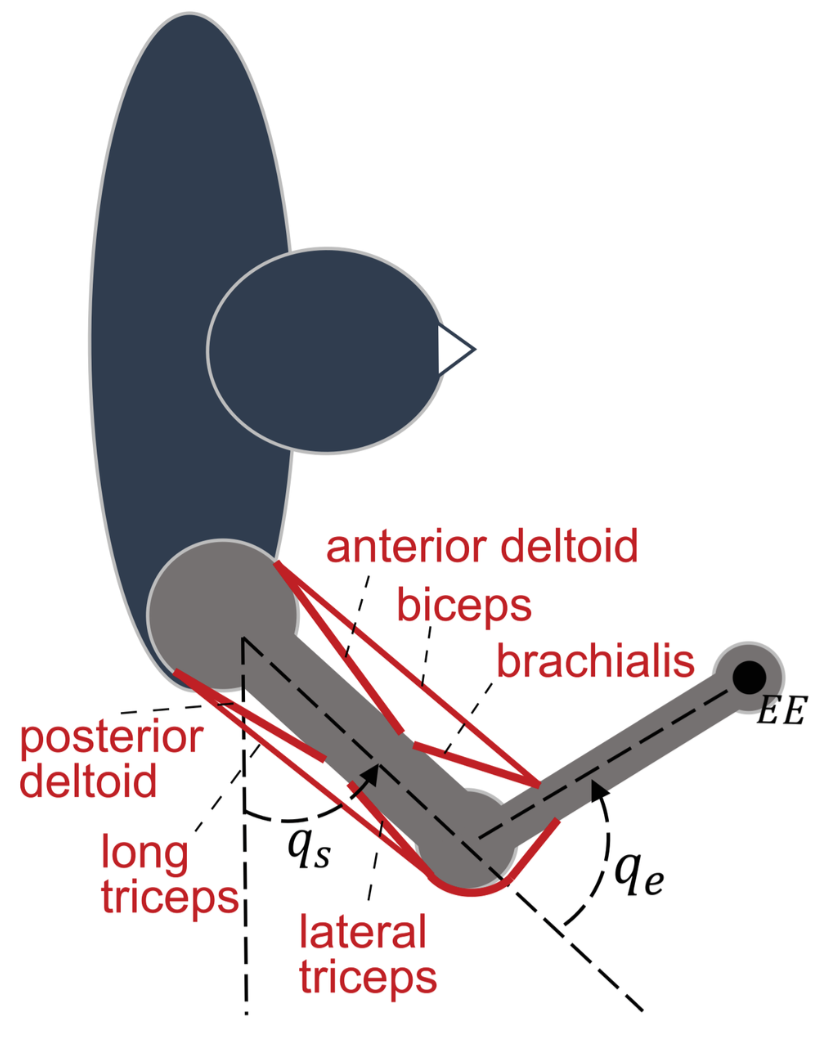
\includegraphics[width=0.5\textwidth]{arm_model_diagram.png}
    \caption{Diagram of the musculoskeletal model of the human arm used in this project \cite{c7}.}
    \label{fig:arm_model}
\end{figure}

The state and control input vectors are defined below:
\begin{align}
    \mathbf{x} &= \begin{bmatrix}
        \mathbf{q} &
        \dot{\mathbf{q}}
    \end{bmatrix}^\top = \begin{bmatrix}
        \theta_s &
        \theta_e &
        \dot{\theta}_s &
        \dot{\theta}_e
    \end{bmatrix}^\top \\
    \mathbf{u} &= \begin{bmatrix}
        a_{\text{brach}} & a_{\text{lattri}} & a_{\text{antdel}} & a_{\text{postdel}} & a_{\text{bic}} & a_{\text{lattri}}
    \end{bmatrix}
\end{align}

Where $\theta_s$ and $\theta_e$ are the shoulder and elbow joint angles, respectively, and $\dot{\theta}_s$ and $\dot{\theta}_e$ are the corresponding joint angular velocities. The control input $\mathbf{u}$ is a vector of muscle activations for each of the 6 muscles in the model. The stochastic dynamics of the system are given by the following differential equation:

\begin{align}
    \dot{\mathbf{x}} &= f(\mathbf{x}, \mathbf{u}, \mathbf{w}) \quad \mathbf{w} \sim \mathcal{N}(0, \Sigma_w) \\
    &= \begin{bmatrix}
        \dot{\mathbf{q}} \\
        M(\mathbf{q})^{-1} \left(C(\mathbf{q}, \dot{\mathbf{q}}) + T_M(\tilde{\mathbf{u}}, \mathbf{q})\right)
    \end{bmatrix} \\
    \tilde{\mathbf{u}} &= \mathbf{u} + \text{diag}(\mathbf{u}) \cdot \mathbf{w}
\end{align}

Where $M(\mathbf{q})$ is the mass matrix of the arm model, $C(\mathbf{q}, \dot{\mathbf{q}})$ is the term describing the Coriolis forces, and $T_M(\mathbf{u}, \mathbf{q})$ is the term describing the torques generated by the muscles. Further details on the dynamics of the system can be found in \cite{c7}.

Following the work of \cite{c7}, we approximate the stochastic state trajectories of the system as normally distributed trajectories. This allows us to represent the stochastic state trajectory as a mean trajectory $\mathbf{x}_\mu(t)$ and a covariance trajectory $P(t)$. We can then use this representation to create a deterministic approximation of the dynamics: 

\begin{align*}
    \dot{\mathbf{x}}_\mu(t) &= f(\mathbf{x}_\mu(t), \mathbf{u}(t), 0) \\
    \dot{P}(t) &= A(t)P(t) + P(t)A(t)^\top + C(t) \Sigma_w C(t)^\top \\
    &\quad A(t) = \frac{\partial f}{\partial \mathbf{x}}\bigg|_{\mathbf{x}_\mu(t), \mathbf{u}(t), 0} \\
    &\quad C(t) = \frac{\partial f}{\partial \mathbf{w}}\bigg|_{\mathbf{x}_\mu(t), \mathbf{u}(t), 0}
\end{align*}

\subsection{Trajectory Optimization}
To plan the trajectory of the arm during a reaching task, we aimed to solve the following optimal control problem:
\begin{align}
    \arg\min_{\mathbf{u}(t)} &\quad \int_0^{t_f} \mathbf{u}(t)^\top R \mathbf{u}(t) dt + k_t \cdot t_f \label{eq:cost} \\
    \text{subject to} &\quad \dot{\mathbf{x}}_\mu(t) = f(\mathbf{x}_\mu(t), \mathbf{u}(t), 0), \quad \mathbf{x}_\mu(0) = \mathbf{x}_0 \label{eq:dynamics_constraint} \\
    &\quad \dot{P}(t) = A(t)P(t) + P(t)A(t)^\top + C(t) \Sigma_w C(t)^\top, \quad P(0) = P_0 \label{eq:dynamics_constraint_p} \\
    &\quad \dot{\mathbf{x}}_\mu(0) = 0, \quad \dot{\mathbf{x}}_\mu(t_f) = 0 \label{eq:boundary_constraints} \\
    &\quad F_k(\mathbf{x}_\mu(t_f)) = \mathbf{p}_{\text{target}} \label{eq:target_constraint} \\
    &\quad [HP(t_f)H^\top]_{i,i} \leq \sigma_{\text{target}, i}^2, \quad H = \frac{\partial F_k}{\partial \mathbf{x}}\bigg|_{\mathbf{x}_\mu(t_f)}, \quad i = 1, \ldots, n \label{eq:target_variance_constraint}
\end{align}

Where $t_f$ is the duration of the trajectory, $R$ is a weight matrix for muscle activations, $k_t$ is a weight for duration, $\mathbf{x}_0$ is the initial state of the arm, $P_0$ is the initial state covariance, $F_k$ is the arm forward kinematics function, $\mathbf{p}_{\text{target}}$ is the position of the target, and $\sigma_{\text{target}, i}$ is the desired standard deviation of the final position of the $i$th dimension of the target.

Equation \ref{eq:cost} works to minimize muscle activations and trajectory duration. Equations \ref{eq:dynamics_constraint} and \ref{eq:dynamics_constraint_p} enforce the dynamics of the system. Equation \ref{eq:boundary_constraints} enforces zero velocity and acceleration at the beginning and end of the trajectory, while equation \ref{eq:target_constraint} enforces the final mean position of the arm's end effector to be at the target. Finally, equation \ref{eq:target_variance_constraint} enforces the final position of the arm's end effector to be within a certain standard deviation of the target position. This standard deviation can be adjusted to model variation in target size in order to test the speed accuracy tradeoff.

\section{Current approach and Results}

\subsection{Existing Model Adaptation}
We initially invested a significant amount of time into adapting the complex 47 muscle OpenSim model for use in our project. However, this model and its supporting trajectory optimization code was developed using a heavily outdated version of OpenSim that is no longer well supported. An attempt was made to transition the model and supporting code to the latest version of OpenSim by adapting to the latest API, but this proved extremely time consuming and difficult to debug due to the complexity of the OpenSim library. As a result, we decided to abandon this model in favor of a simpler model.

\subsection{Modeling Signal Dependent Motor Noise}
The decision to combine noise into a trajectory optimization model meant we needed to find more information on modeling signal dependent noise. This led to the frequently referenced model by Harris and Wolpert \cite{c2}. This model applied white noise to the neural command signal that activates muscles. The noise is increased proportionally to the control signal strength. In order to add noise into a trajectory optimization model, we began researching other potential models which combined both noise and trajectory optimization. This lead us to the model by Todorov and Li \cite{c8}, which uses an iterative LQG model for locally-optimal feedback control which incorporates control dependent noise. Todorov found the control dependent noise has a similar effect to an energy cost, and utilized a stochastic model of the human arm with six muscle actuators in their model. Their work was further iterated on by Van Wouwe et al. \cite{c7}, who determined that the iLQG model required assumptions and tuning which might not be physically realistic. They acknowledged that the hand tuned cost functions were a simplifaction that potentially sacrificed accuracy. As a result, the Van Wouwe model uses stochastic simulations for both feedforward and feedback control their nonlinear musculoskeletal model, which also uses six muscles. 

We immediately recognized the potential usefulness of this model, as it was implemented in MATLAB and was freely available on github. As a result, when we decided to transition away from using the complex 47 muscle model, it was a clear choice to make. The model already included a framework for modeling reaching trajectories in the presence of both signal and motor noise, and although it was not geared towards analyzing the speed accuracy tradeoff it would not be overly difficult to adapt it for that purpose. We also considered using the model proposed by Peternel, et al. \cite{c9}, which also examined stochastic optimization in the presence of motor noise, while also focusing on the speed accuracy tradeoff. However, this model was not readily avaliable to download, so we decided against attempting to recreate it in favor of adapting the Van Wouwe model.

\subsection{Trajectory Optimization using Direct Colocation}
Working with the Van Wouwe model, we adapted the optimal control framework from \cite{c7} to only perform feed forward control and to fit our trajectory optimization problem. This implementation required us to discretize the muscle activation trajectory into a vector of $N$ nodes, and to optimize over that vector. To enforce the dynamics efficiently, we use a method referred to as direct colocation. This involves similarly discretizing the state trajectory into a series of $N$ nodes that are added to the design vector, and then enforcing the dynamics constraints between each consecutive node. This formulation results in the following design vector:

\begin{align}
    \mathcal{X} &= \begin{bmatrix}
        \mathbf{u}_1 & \cdots & \mathbf{u}_N & \mathbf{x}_{\mu1} & \cdots & \mathbf{x}_{\mu N} & P_1 \cdots & P_N & t_f
    \end{bmatrix}^\top
\end{align}

Where $\mathbf{u}_i$, $\mathbf{x}_{\mu i}$, and $P_i$ are the muscle activations, state, and state covariance at the $i$th node, respectively. Then the discretized optimization problem can be formulated as follows:

\begin{align}
    \arg\min_{\mathbf{u}} &\quad \sum_{i=1}^{N} \mathbf{u}_i^\top R \mathbf{u}_i + k_t \cdot t_f \label{eq:dcost} \\
    \text{subject to} &\quad \mathbf{x}_{\mu i+1} = \mathbf{x}_{\mu i} + f(\mathbf{x}_{\mu i}, \mathbf{u}_i, 0) \delta t, \ i = 1, \dots, N-1 \\
    &\quad P_{i+1} = (I + A_i \delta t)P_i(I + A_i \delta t)^\top + C_i \Sigma_w C_i^\top \delta t, \ i = 1, \dots, N-1 \\
    &\quad \mathbf{x}_{\mu 1} = \mathbf{x}_0, \quad f(\mathbf{x}_{\mu 0}, \mathbf{u}_0, 0) = 0, \quad f(\mathbf{x}_{\mu N}, \mathbf{u}_N, 0) = 0 \label{eq:dboundary_constraints} \\
    &\quad F_k(\mathbf{x}_{\mu N}) = \mathbf{p}_{\text{target}} \label{eq:dtarget_constraint} \\
    &\quad [HP_NH^\top]_{i,i} \leq \sigma_{\text{target}, i}^2, \quad H = \frac{\partial F_k}{\partial \mathbf{x}}\bigg|_{\mathbf{x}_{\mu N}}, \quad i = 1, \ldots, n \label{eq:dtarget_variance_constraint}
\end{align}

Note at the dynamics of the mean and covariance trajectories are enforced using simple forward Euler integration. We may experiment with different integration methods in the future to improve accuracy.

\subsection{Demo Results}

While we have not completed the implementation of our previously formulated trajectory optimization problem using the Van Wouwe model, we were able to adapt and implement a simplified version of the problem to plan a trajectory for a reaching task. A demo of this simulated trajectory can be found in figures \ref{fig:demo_activations}, \ref{fig:demo_joints}, and \ref{fig:demo_position}. In this demo, we only minimized muscle activations, opting for a fixed time duration of 0.8 seconds. The motor noise was simple Gaussian noise added to the joint torques, rather than signal dependent noise added to the muscle activations; this alternative noise formulation was used because it was already implemented in the model. Finally, a relatively large (and therefore lenient) target position covariance was used in the constraint function to allow for fast optimization trials while debugging. Now that we have the basic implementation working, we will begin adapting our code to address all of these problems.

\begin{figure}[H]
    \centering
    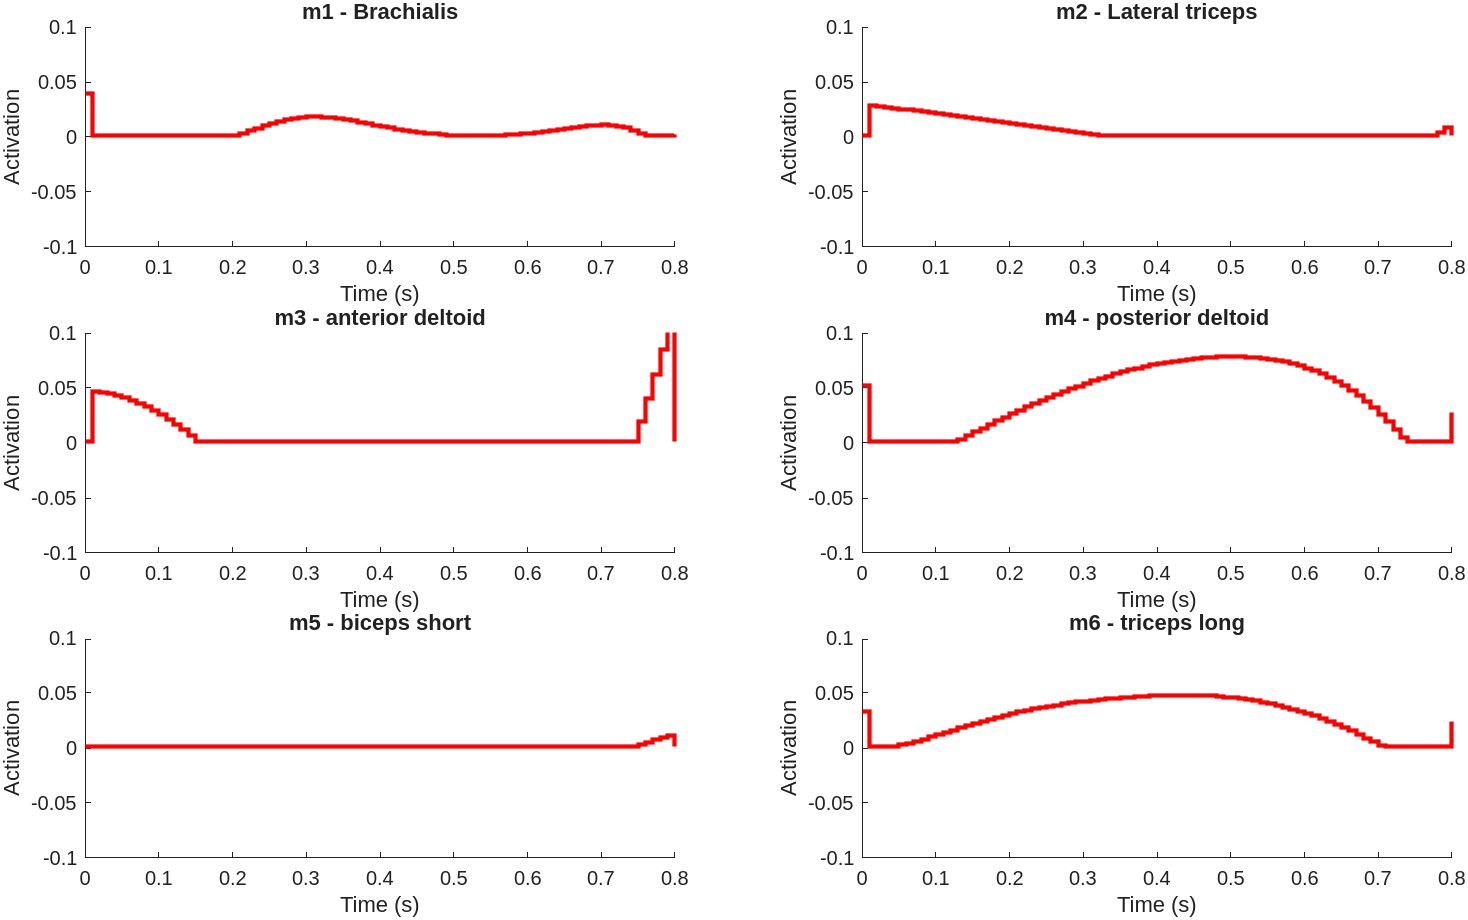
\includegraphics[width=0.8\textwidth]{demo_new_state_activations.jpg}
    \caption{Muscle activation trajectories for a reaching task using the Van Wouwe model.}
    \label{fig:demo_activations}
\end{figure}

\begin{figure}[H]
    \centering
    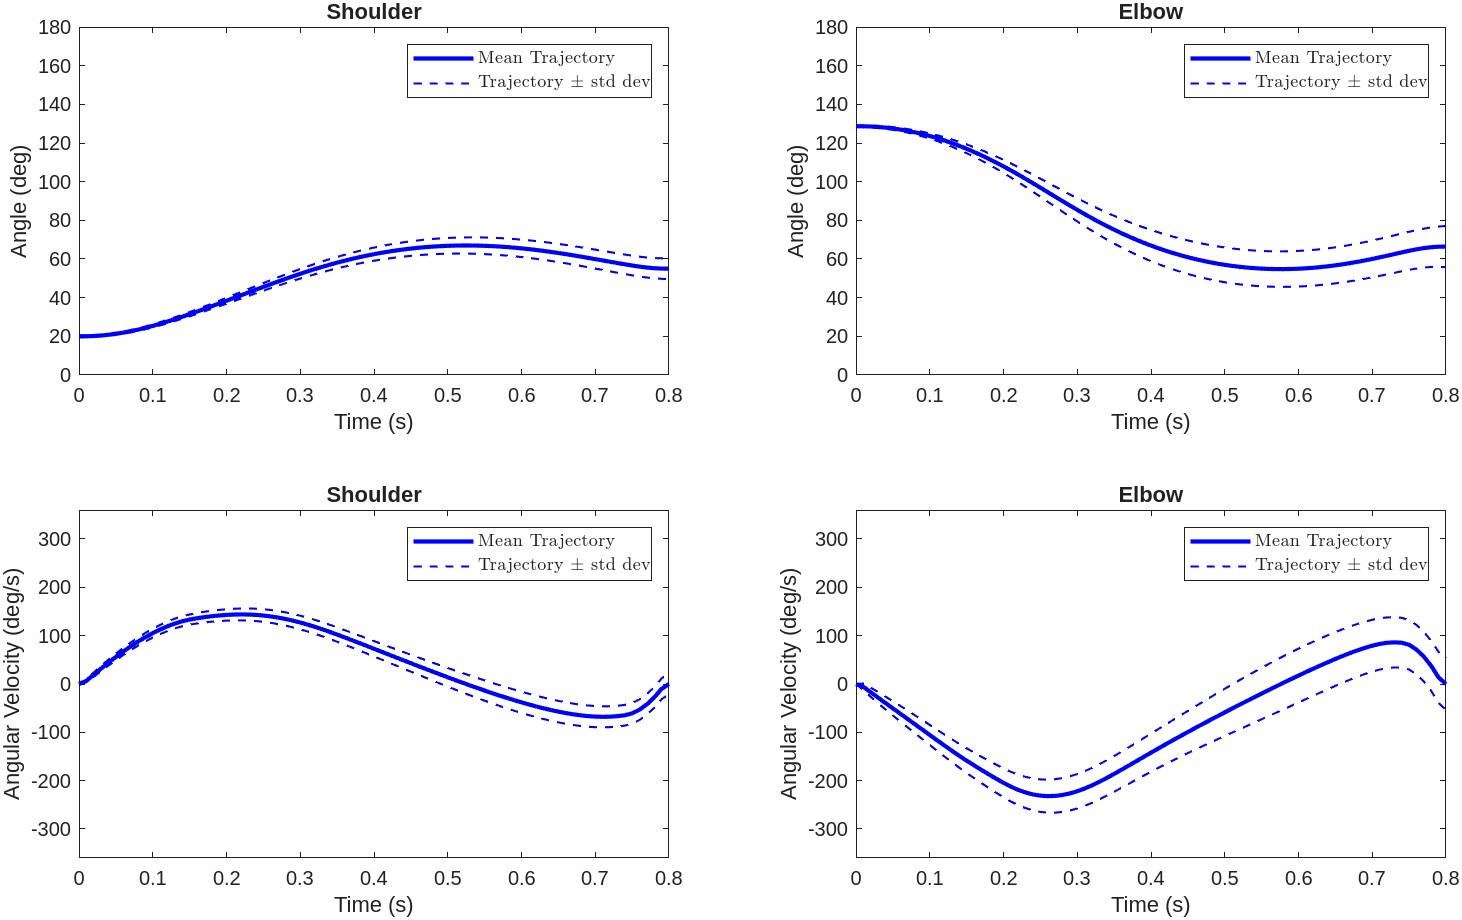
\includegraphics[width=0.8\textwidth]{demo_new_state_joints.jpg}
    \caption{Joint angle and velocity trajectories for a reaching task using the Van Wouwe model.}
    \label{fig:demo_joints}
\end{figure}

\begin{figure}[H]
    \centering
    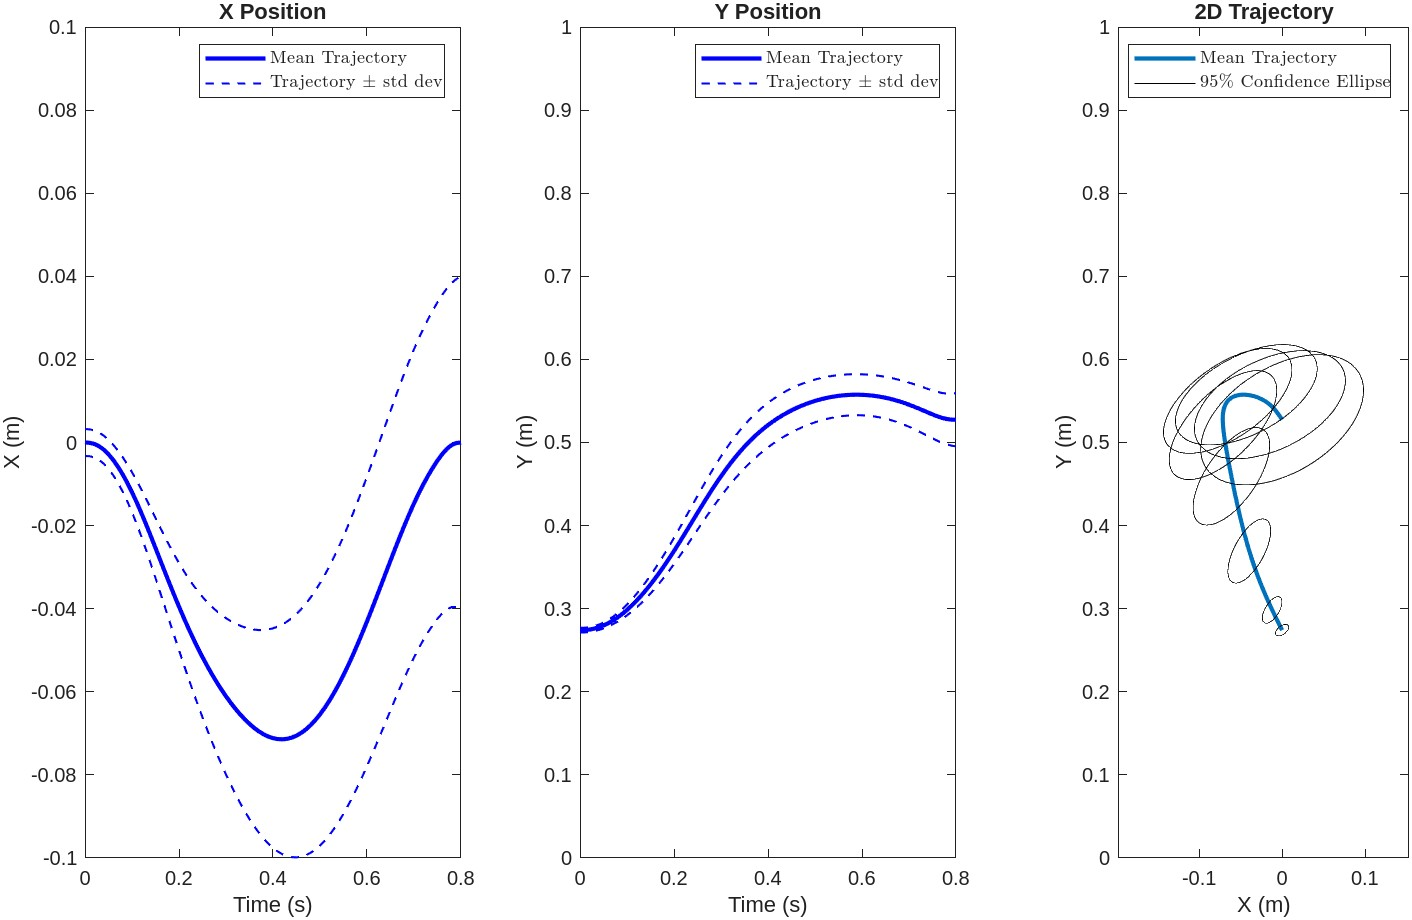
\includegraphics[width=0.8\textwidth]{demo_new_state_positions.jpg}
    \caption{End Effector trajectory for reaching task using the Van Wouwe model. The end effector covariance grows large towards the end of the trajectory because it was very loosely constrained.}
    \label{fig:demo_position}
\end{figure}
\section{Remaining Timeline}
\begin{itemize}

    \item \textbf{3/25} Riley: Ensure the MATLAB model has been sufficiently adapted to model the speed accuracy tradeoff. The model should allow for input of target accuracy and output of movement duration. Begin implementing new trajectory optimization techniques into the model.

    Ethan: Implement signal dependent motor noise generation into the MATLAB model. Begin to unsure output of noise models falls within anticipated variation ranges as described by \cite{c2}.

    \item \textbf{4/1} Riley: Continue testing and iterating on the trajectory optimization implementation, begin running trials and collecting data for metrics, begin planning and preparing background slides for final presentation

    Ethan: Continue to verify the model parameters for both trajectory optimization and noise addition are satisfactory (Dependent on completed formulation and testing in MATLAB), begin planning and preparing background slides for final presentation.

    \item \textbf{4/8} Riley: Continue running trials and collecting data for metrics, begin analysis of collected data, continue preparing slides for final presentation.

    Ethan: Continue testing and iterating on the trajectory optimization implementation, begin running trials and collecting data for metrics, continue preparing slides for final presentation.

    \item \textbf{4/15} Riley: Finish analysis of collected data, finish final presentation, begin final report.

    Ethan: Finish running trials and collecting data for metrics, finish final presentation, begin final report.

    \item \textbf{4/22 (Final Report)} Riley: Finish final report.

    Ethan: Finish final report.

\end{itemize}
% \subsection{Anticipated Challenges}
% One of the main challenges we anticipate to complexity of the model we intend to use for simulation. This model is a high fidelity biologically accurate model of the human arm including 47 muscle-tendon actuators and 5 degrees of freedom. This complexity may cause our optimal control simulations to be prohibitively slow to run, and it may make it difficult to implement the signal-dependent motor noise. If we encounter these problems, we plan to instead use a simplified human arm model with fewer actuators. This may reduce our ability to accurately replicate human behavior, but it will allow us to complete the project in a reasonable amount of time.

% Another challenge we anticipate is use of the OpenSim simulation software and C++ programming language. Neither of us have experience using OpenSim, so it is possible that there will be very significant learning curve to overcome, or even that it will lack features we need in order to complete the project. Although we both have experience using C++, we have never used it for optimal control. Because this use case often requires well developed libraries and optimization tools (e.g. fmincon in MATLAB) in order for rapid prototyping and testing to be feasible, we may encounter significant difficulty in implementing our optimal control simulations in C++ if these tools and libraries are not available. If we encounter these problems, we plan to use MATLAB instead of C++ for the optimal control simulations. MATLAB is known to have a well developed set of tools for use with trajectory optimization, and one of us has direct experience using it for that purpose. If this prevents us from using the original complex model, we will use a simplified model as described above.



\section{Goals and Evaluation}
Our original baseline goal for this project was to modify the simulation and control method from the original paper to include signal-dependent motor noise and produce a meaningful comparison between the these new simulated results and experimental data collected from previous studies. As a result of the challenges encountered with utilizing this existing model, we have decided to change course slightly. Our goal now has shifted to now adapt the trajectory optimization model from Van Wouwe. Our final goals for the project remain the same for this model in relation to implementation of motor noise and additional trajectory optimization methods, but they will now be applied to a less complex model in the more familiar MATLAB environment. This will greatly improve the ease of use of the model and allow us to work more quickly towards our goals of implementing and modifying the model. Specifically, we will consider this project successful if we are able to do the following:
\begin{itemize}
    \item Incorporate signal dependent motor noise into our simulation in a way that is, at least in some aspects, biologically realistic and backed up by previous literature. We will implement Gaussian noise proportional to the actuator command strength.
    \item Run this simulation and collect data from a sufficient number of trials (at least 10) for each reaching task described in the Problem Description section. 
    \item Analyze the collected data and compare it to experimental data from previous studies (Specifically from the paper Al Borno, et al for optimization comparison and Harris and Wolpert for noise comparison) and to correlate our results with Fitt's Law, using the metrics described in the Problem Description section. 
\end{itemize}

As an additional stretch goal, we aim to compare the results of the original trajectory optimization method used in the original paper to the results of an alternative trajectory optimization method. Specifically, we will consider this goal successful if we are able to do the following:
\begin{itemize}
    \item Choose an alternative trajectory optimization method and implement it into our simulation.
    \item Run the simulation and collect data from a sufficient number of trials (at least 10) for each reaching task described in the Problem Description section using the alternative trajectory optimization method(s).
    \item Analyze the collected data and compare it to the original trajectory optimization method using the metrics described in the Problem Description section.
\end{itemize}

\begin{thebibliography}{99}
\bibitem{c1}
Fitts PM (1954) The information capacity of the human motor system in controlling the amplitude of movement Journal of Experimental Psychology 47:381–391. https://doi.org/10.1037/h0055392 

\bibitem{c2}
Harris, C., Wolpert, D. Signal-dependent noise determines motor planning. Nature 394, 780–784 (1998). https://doi.org/10.1038/29528

\bibitem{c3}
Heitz RP (2014) The speed-accuracy tradeoff: history, physiology, methodology, and behavior Frontiers in Neuroscience 8:150. https://doi.org/10.3389/fnins.2014.00150

\bibitem{c4}
Lillicrap TP, Hunt JJ, Pritzel A, Heess N, Erez T, Tassa Y, Silver D, Wierstra D (2015) Continuous control with deep reinforcement learning arXiv. https://arxiv.org/abs/1509.02971

\bibitem{c5}
Mazen Al Borno, Saurabh Vyas, Krishna V Shenoy, Scott L Delp (2020) High-fidelity musculoskeletal modeling reveals that motor planning variability contributes to the speed-accuracy tradeoff 
https://doi.org/eLife 9:e57021

\bibitem{c6}
Trivedi U, Menychtas D, Alqasemi R, Dubey R. Biomimetic Approaches for Human Arm Motion Generation: Literature Review and Future Directions. Sensors (Basel). 2023 Apr 12;23(8):3912. doi: 10.3390/s23083912.

\bibitem{c7}
Van Wouwe T, Ting LH, De Groote F (2022) An approximate stochastic optimal control framework to simulate nonlinear neuro-musculoskeletal models in the presence of noise. PLOS Computational Biology 18(6): e1009338. https://doi.org/10.1371/journal.pcbi.1009338

\bibitem{c8}
E. Todorov and Weiwei Li, "A generalized iterative LQG method for locally-optimal feedback control of constrained nonlinear stochastic systems," Proceedings of the 2005, American Control Conference, 2005., Portland, OR, USA, 2005, pp. 300-306 vol. 1, doi: 10.1109/ACC.2005.1469949.

\bibitem{c9}
Peternel L, Sigaud O and Babič J (2017) Unifying Speed-Accuracy Trade-Off and Cost-Benefit Trade-Off in Human Reaching Movements. Front. Hum. Neurosci. 11:615. doi: 10.3389/fnhum.2017.00615



\end{thebibliography}
\end{document}

